
% Luigi Coniglio 
\subsection{En-tête IPv4}
Un paquet IPv4 est precedé par un en-tête ayant une longueur minimale de 20 octets 
(dans les cas où aucune option supplémentaire a été specifiée).
La figure suivante montre le contenu de l'en-tête d'un paquet IPv4.


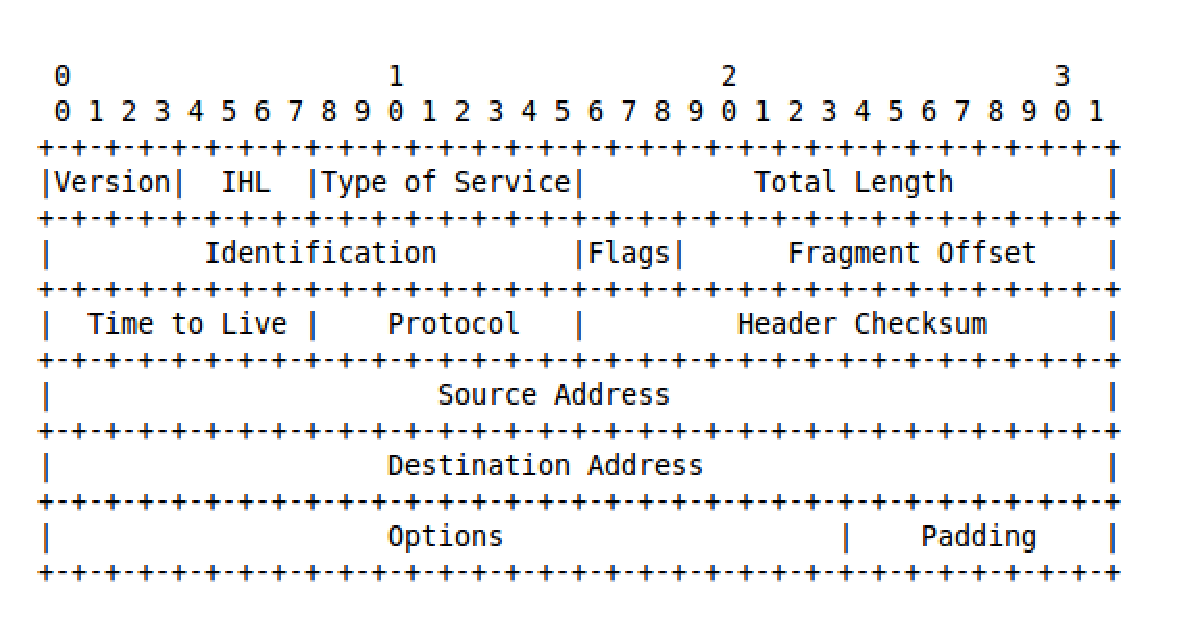
\includegraphics[width=15cm]{./pics/IPv4header.eps}


Comme on peut le voir dans la figure ci-dessus, un en-tête IPv4 est composé, en plus le padding, de
13 champs. En réalité nous verrons plus loin que cet en-tête
peut, quand c'est nécessaire, contenir un champ additionnel grâce auquel
on peut spécifier quelques options qui ne sont pas présentes dans les 13 champs
au dessus.


Commencons par voir en detail les 13 champs d'un en-tête IPv4 standard:

\begin{description}
\item [Version] 
Ce champ occupe les 4 premiers bits de l'en-tête IPv4.\\
Il est utilisé pour déterminer le type de protocole utilisé par la couche
réseau (couche 3). Dans le cas de IPv4 ce champs contiendra toujours la valeur
4, qui identifie le protocole IPv4.

Ce champ n'est positionné par hasard dans l'en-tête. En effet, pour
connaître la position des autres champs de l'en-tête, il faut d'abord savoir
quel est le protocole utilisé et donc le type de l'en-tête.
En pratique, dans la plupart des cas ce champ n'est pas très utile, car le
protocole à utiliser pour la couche 3 est souvent spécifié dans l'en-tête du
protocole de la couche liason.

\item [IHL]
Le champ IHL (acronime de Interet Header Length) specifie la taille de l'en-tête IPv4. 
Bien entendu, en disant cela on souligne un concept important du protocole IPv4: 
la taille de l'en-tête n'est pas fixe.

La taille de l'en-tête est exprimée en blocs de 32 bits. Étant donné une taille de
4 bits pour le champ IHL, la longueur maximale d'un en-tête IPv4 est de 15 blocs de
32 bits, ce qui correspond à 60 octets. Comme l'en-tête IPv4 a une taille minimale
de 20 octets (160 bits), le champ IHL ne peut pas contenir une valeur inférieure à 5.

\item [Type of Service]
Le champ Type of Service, mieux connu sous l'acronime ToS, est utilisé pour 
spécifier la qualité de service souhaité pour l'envoie d'un paquet IPv4.
Ce champ occupe un octet de l'en-tête et il est composé de trois parties.
Une première partie de 3 bits permet d'indiquer la priorité avec laquelle
le paquet doit être traité, les 3 bits suivants sont utilisés pour spécifier 
certaines caractéristiques du service, notament: le temps, le débit et la fiabilité.
Enfin, les deux derniers bits n'ont pas été utlisés et leur signification a été 
réservée pour des implémentations futures.

En realité l'histoire de ces champs est bien plus longue et complexe,
car en pratique la façon d'utiliser ces champs a ete modifée plusieurs fois au 
cours des années.
\footnote{L'utilisation des 8 bits du champ ToS a été redéfinie
par cinq standard différents (plus divers standards experimentaux).
Les documents présentant ces standards sont mentionnés dans le chapitre 
"Historical Definitions for the IPv4 TOS Octet" du RFC 3168}
Ce manque de stabilité a parfois causé une certaine confusion lors des différentes implementations.
\footnote{Comme le souligne le RFC 3260 {\it "At least one implementor has expressed confusion about the
relationship of the DSField, as defined in RFC 2474, to the use of
the TOS bits, as described in RFC 1349"}}

Aujourd'hui les 8 bits du champ ToS sont utilisés par le mécanisme DiffServ
(Differentiated Services). Ce système utilise les premiers 6 bits du champ
ToS (DSCP - Differentiated Services Code Point) pour marquer chaque paquet
comme appartenant à un niveau de priorité et à une classe de service. Chaque
classe détermine le type de traitement que doivent effectuer les routeurs que le paquet traverse
 (PHB - Per-Hop behaviour), toutefois le service offert
par chaque router est fortement lié à sa configuration.
\footnote {
{\it "The DiffServ standard does not specify a precise definition of "low," "medium,"
and "high" drop probability. Not all devices recognize the DiffServ (DS2 and
DS1) settings; and even when these settings are recognized, they do not
necessarily trigger the same PHB forwarding action at each network node. Each
node implements its own response based on how it is configured."} - 
Implementing Quality of Service Policies with DSCP
http://www.cisco.com/c/en/us/support/docs/quality-of-service-qos/qos-paquet-marking/10103-dscpvalues.html}
Les 2 derniers bits du champ ToS sont utilisés pour l'extension ECN ({\it Explicit Congestion
Notification }). Cette extension, proposée par le RFC2481n et introduite deux années plus tard par le RFC3168,
ajoute un système de contrôle de la congestion du trafic réseau. Dans le cas d'une saturation
du réseau, ce champ est utilisé pour notifier ce problème et demander au dispositif émetteur
une réduction du rythme auquel les paquets sont envoyés, afin de réduire l'attente et
la perte de paquets.

\item [Total length]
Comme le suggère son nom, ce champ est utilisé pour indiquer la taille totale du
paquet IPv4: en-tête + données. Le champ {\it Total length} est défini sur 16
bits, ce qui permet d'indiquer une valeur comprise entre 0 et 65 535 octets. Comme l'en-tête
est compris dans la longeur totale d'un paquet, cette valeur ne sera jamais inférieure
à 20 (taille minimale d'un en-tête IPv4 en octets).
Le RFC 791 impose à tous les dispositifs d'un réseau IPv4 la capacité de recevoir
des paquets d'une taille maximale de 576 octets, cette prérogative permet d'éviter une fragmentation excessive.

\item [Identification]
Cet en-tête (sur 16 bits) permet d'identifier les fragments appartenant au même paquet.

\item [Flags]
Les 3 bits du champ Flags sont utilisés pour gérer la fragmentation d'un paquet.
Un de ces bits est utilisé pour indiquer si le paquet peut être fragmenté ou
non. Ce bit, appellé DF ({\it Don't Fragment}), doit être pris en considération
par les routeurs sur le chemin du paquet pour décider si un paquet est trop grand pour être
trasmit ou s'il doit être retrasmit sous forme de fragments plus petits ou s'il doit être rejeté. 
Un autre bit, appellé MF ({\it More Fragments}), indique si le paquet est suivi 
par d'autres fragments. Le bit MF est mis à 0 dans le dernier fragment ou dans
des paquets qui n'ont pas été fragmentés.

Un des trois bits de ce champs n'est pas actuellement utilisé mais il a été
réservé pour des applications futures possibles.
\footnote {Ce bit a aussi été le protagoniste d'un des plus connu poissons
d'avril presentés par l'IETF. Pour faciliter les tâches des systèmes de filtrage 
le RFC 3514 propose d'utiliser ce bit pour étiqueter les paquets mailveillants et à ce
titre tous les paquets étant envoyés avec ce bit (renomme "{\it Evil Bit}") 
mis a 1 seraient mis à la poubelle.}

\item [Fragment Offset]
Lorsque un paquet a été fragmenté cet en-tête est utilisé pour déterminer la
position (offset) d'un fragment par rapport à l'ensemble des du paquet réassemblé.
Le décalage de chaque fragment est exprimé en blocs de huit octets (ou 64
bits). Le champ Fragment Offset utilise 13 bits de l'en-tête IPv4, ce qui permet
un offset maximale de 65,528 octets.\footnote {En pratique un tel offset n'est
jamais utilisé car, en ajoutant un en-tête minimale de 20 octets, la taille
totale du paquet réassemblé dépasserait la longueur maximale d'un paquet IPv4.}
Étant donné que le flag MF ({\it More Fragments}) doit être mis à zero lorsqu'un paquet 
n'est pas fragmenté, ou si il est le dernier fragment d'un paquet plus grand, 
l'unique différence entre ces deux types de paquets est la valeur du 
champ Fragement Offset qui, dans le cas d'un paquet non fragmenté, est
toujours zero.

\item [Time to Live]
Ce champ détermine le nombre maximal de fois qu'un paquet peut être retrasmit, 
il est utilisé pour empêcher qu'un paquet puisse être retrasmis à l'infini.
Chaque routeur le long du chemin d'un paquet regarde la valeur du champ. Si la 
valeur a atteint 0, il détruit le paquet, et sinon il décrémente le champ par le
nombre de secondes que le paquet passe en attente avant qu'il soit trasmis.

En théorie, le TTL indique le nombre de secondes pendant lesquelles un paquet
peut continuer à être retrasmis dans un réseau, mais un routeur 
 décrémente toujours ce champ d'au moins 1 (même si le paquet a été
retrasmis en moins d'une seconde) et, en considérant les performances des routeurs
d'aujourd'hui, le TTL indique en pratique le nombre maximum de routeur qu'un paquet
 peut traverser au cours de son achemiminement.

L'espace reservé au TTL dans l'en-tête IPv4 est d'un octet, ce qui veut dire qu'on a un 
TTL maximum de 255.\footnote {Le RFC 1700 recommende une valeur par défaut de 64.}

Quand un paquet a été détruit suite à l'expiration du TTL, le routeur qui a
détruit le paquet peut décider d'envoyer un message d'erreur a l'émetteur du
paquet détruit. Ce type de message (ICMP Time exceeded) est également utilisé par
utils comme {\it traceroute} pour découvrir, approximativement, le chemin 
d'un paquet IP.

\item [Protocol]
Chaque paquet IPv4 spécifie le protocole utilisé par les données transmises:
cela est l'objectif de ce champs de 8 bits 

\item [Header Checksum]
Ce champ contient une somme de contrôle et est utilisé pour détecter des 
erreurs dans l'en-tête IPv4. La valeur de ce champ est recalculé à
chaque retrasmission\footnote {Cela est nécessaire car le TTL est décrementé
à chaque retrasmission et un changement de l'en-tête amène à une valeur différente
dans la somme de contrôle}: si la somme de contrôle ne correspond pas avec celle 
présente dans l'en-tête du paquet, celui-ci est detruit.


\item [adresse source et adresse destination]
Les adresses de chaque paquet IPv4 (soit l'adresse source et l'adresse de
destination du paquet) sont représentés sous forme d'une suite de 32 bits.

L'adresse source de chaque paquet représente dans la plupart des cas
l'adresse logique\footnote {Il ne faut surtout pas oublier la différence entre
une adresse physique, comme par exemple une adresse MAC (qui est liée a
l'hardware et est donc unique pour chaque machine), et une adresse logique,
comme par exemple une adresse IP (qui peut changer et identifie une machine
dans un réseau en particulier).} de la machine qui a envoyé le paquet
(à laquelle il faudra donc éventuellement répondre).  Dans certains cas,
 cette adresse ne correspond pas à celle de la machine qui a envoyé
le paquet, c'est par exemple ce qui se passe dans une requête, {\it ARP probe}
lorsque la valeur de l'adresse de la machine source est 0.0.0.0 (ce qui represente
une adresse indéfinie\footnote {Notex que la signification de l'adresse 0.0.0.0
est liée à la façon dont elle est utilisée. En general elle indique {\it aucune
adresse en particulier}. 

Dans la plupart des cas, cette adresse est utilisée
pour indiquer une de ces valeurs: l'adresse de la machine courante (c'est
l'adresse de loopback), n'importe quelle adresse ou réseau (c'est le cas de la
route par default dans une table de routage), une adresse indéfinie ou bien une
combinaison des possibilitées précédentes (c'est le cas d'une requête {\it ARP
probe} ou bien d'une requête {\it DHCP Discovery} ou {\it DHCP Request}, ou
 l'adresse source 0.0.0.0 indique une adresse indéfinie mais aussi l'adresse
de la machine actuelle, que del reste n'est pas encore defini...).}
) car elle n'a pas encore déterminée son adresse IP. 

L'adresse de destination d'un paquet IPv4 identifie la machine vers
laquelle le paquet doit être expedié. Comme dans le cas de l'adresse source,
 l'adresse de destination peut aussi contenir des valeurs speciales. En effet, certaines 
valeurs puvent être utilisée par exemple pour identifier plusieurs machines
(adresses multicast), toutes les machines d'un réseau (adresse de broadcast) ou
la machine actuelle (adresse de loopback).

Une description plus detaillée des mécanismes liées aux adresses IPv4 est
proposée dans le chapitre  
%TODO mettre chapitre% 
de ce rapport.


\item [Options] 
Ce champ n'est pas obligatoire et il peut donc ne pas être présent dans un
en-tête IPv4. La présence de ce champ est déterminé par la valeur du
IHL: lorsque cette valeur indique une taille de l'en-tête IPv4 supérieure à 
la taille minimale (20 octets), l'en-tête contiens des options.
Étant donné qu'un en-tête IPv4 peut avoir une taille maximale de 
60 octets (la valeur du IHL est égal à 15), le champ Options peut occuper
40 octets au meximum.

Ce champ a été conçu pour étendre les possibilitées de IPv4 en ajoutant des fonctions
extra.  Aujord'hui il y a quelque dizaines d'options qui ont été
specifiées\cite{url-optsIPv4} (si on considère également les options experimentales)
mais peut d'entre elles sont réelement utilisées. Parmi les options les plus connues
on retrouve par exemple des ajouts utiles à l'administration et au debuggage
d'un réseau, comme {\it Record route} qui permet d'enregistrer les adresses
des routeurs dans le chemin d'un paquet IP, et {\it Timestamp} qui permet de
savoir le temps passe entre chaque saut du chemin.

Parmi les options il en y a deux qui ont une fonction spéciale: EOL 
({\it End Of Option List}) and NOP ({\it No Operation}): l'option EOL 
est utilisée pour indiquer la fin de la chaîne d'options, NOP est une option
sans aucun effet, elle est utilisée comme remplissage pour aligner les options 
quand elles ne sont pas alignées sur 4 octets\footnote {On rappelle que 
le champ IHL indique la longuer de l'en-tête IPv4 en blocs de 32 bits 
(4 octets)}.



\item [Padding] 
Le padding ne contient que des zéros et est utilisé quand la fin de l'en-tête
n'est pas aligné sur 32 bits (4 octets). Bien entendu, ce champ est optionnel:
en effet, il peut être necessaire seulement lorsque l'en-tête IPv4 termine avec
une option dont la limite n'est pas alignée sur 32 bits. Un en-tête d'un paquet IPv4 
de 20 octets (donc sans aucune option) n'a besoind'aucun Padding car il est aligné sur
4 octets (20 étant un multiple de 4)
\end{description}
